% !TeX spellcheck = ru_RU
% !TEX root = vkr.tex

\section{Система бенчмарков}

Бенчмарки в репозитории проекта \verb|tokio| не пригодны для анализа производительности в рамках данной работы, так как используют методы синхронизации имеющие нетривиальный эффект на результатах экспериментов:

\begin{itemize}
    \item Атомарное чтение и запись из множества исполняемых разными потоками задач скорее позволяет измерять производительность системы памяти физической машины, нежели взаимодействия структур рантайма~\cite{atomicOnModerHardware}.
    \item Ожидание исполнения в методе \verb|block_on| \verb|tokio| рантайма чревато неточным измерением из-за текущей реализации\footnote{\href{https://github.com/bheisler/criterion.rs/issues/819}{Проблема} измерения производительности асинхронных функций (Дата обращения: 25.5.2025)}.
\end{itemize}

Поэтому в качестве системы бенчмарков был создан проект \verb|tokiobench|\footnote{\href{https://github.com/IgorErin/tokiobench}{Репозиторий} проект tokiobench (Дата обращения: 25.5.2025)}, где предполагалось реализовать сценарии использования проекта \verb|tokio| в \verb|TATLIN.BACKUP|. При общении с командой \verb|TATLIN.BACKUP| был выделен основной сценарий, представленный на рисунке~\ref{fig:scenario}:

\begin{figure}[H]
    \begin{center}
        \makebox[\textwidth]{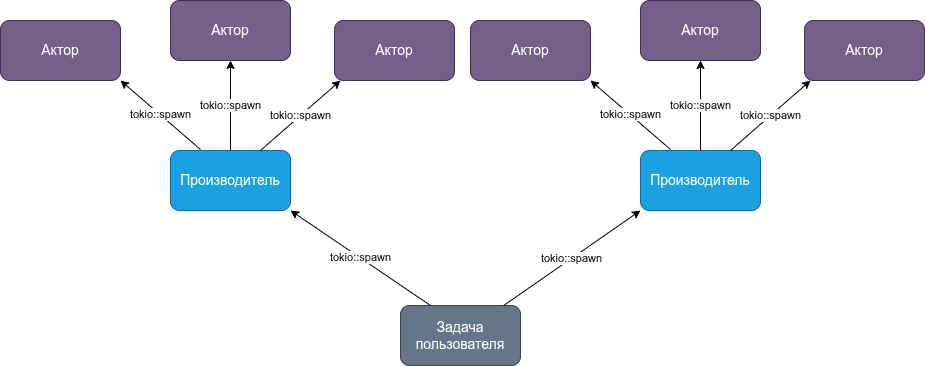
\includegraphics[scale=0.55]{pictures/scenario.drawio.png}}
    \end{center}

    \caption{Основной сценарий использования tokio в TATLIN.BACKUP.}
    \label{fig:scenario}
\end{figure}

\begin{itemize}
    \item Актор --- замыкания, в цикле ожидающие асинхронные события.
    \item Производитель --- замыкания, отправляющее на исполнение множество замыканий акторов.
\end{itemize}

Необходимо было исследовать производительность такого сценария при следующих параметрах:

\begin{itemize}
    \item Тысяча замыканий акторов.
    \item Тысяча итераций исполнения акторов.
    \item Сто замыканий производителей.
\end{itemize}

\subsection{Реализация бенчмарков}

Бенчмарки \verb|tokio| не предполагают измерения производительности, а призваны лишь отслеживать регрессии при изменениях исходного кода. Поэтому в \verb|tokiobench| реализуются бенчмарки со следующими изменениями:

\begin{itemize}
    \item атомарныя переменная была заменена иерархией преаллоцированных буферов, переиспользуемых от итерации к итерации и коллекционирующих структры типа \verb|JoinHandle|;
    \item ожидание структур типа \verb|JoinHandle| перенесено из текущего потока с методом \verb|block_on| в отдельную задачу, которая сообщает о завершении обработки с помощью блокирующего канала.
\end{itemize}

Все это призвано сократить наблюдаемые эффекты от реализации системы бенчмаркинга.

Использование блокирующего канала приводит к появлению дополнительных накладных расходов. Для их учета была создана реализация использующая спинлок: фиксирующий исполнение и сигнализирующий поток пишет значение в атомарную переменную, поток бенчмарка ожидает этого в цикле.

Для эмуляции операций ввода вывода был использован метод \verb|yield_now()|. А именно, каждый актор тысячу раз выполняет \verb|yield_now()|, что заставляет исполнителя сохранять структуру типа \verb|Waker| в локальной коллекции, для последующего вызова метода \verb|wake()|. После чего вызов метода \verb|wake()| приводит к переполнению локальной очереди исполнителя, вынуждая последнего перемещать задачи из локальной очереди в глобальную. После исполнения задач из локальных очередей исполнители начинают обращаться к глобальной очереди, затем похищают задачи друг у друга. Такая реализация приводит к повышению числа взаимодействий у исполнителей, что способствует более объективной оценке накладных расходов этого взаимодействия.
